\documentclass[11pt,a4paper]{article}
\usepackage[margin=25mm]{geometry}
\usepackage[T1]{fontenc}
\usepackage{lmodern}
\usepackage{amsmath,amssymb,amsthm}
\usepackage{graphicx}
\usepackage{microtype}
\usepackage[hidelinks]{hyperref}

\hypersetup{
  pdftitle={A rectangle interpretation of Vieta jumping for IMO 1988 Problem 6},
  pdfauthor={Pranay Manocha},
  pdfsubject={An expository note on an area interpretation of integer descent},
  pdfkeywords={Vieta jumping, infinite descent, Diophantine equations, IMO 1988}}
\newtheorem{theorem}{Theorem}
\newtheorem{lemma}[theorem]{Lemma}
\newtheorem{corollary}[theorem]{Corollary}
\setlength{\emergencystretch}{2em}
\raggedbottom

\title{A rectangle interpretation of Vieta jumping\\
  for IMO 1988 Problem 6}
\author{Pranay Manocha\\[3pt]\small Independent researcher}
\date{19 September 2026\\[3pt]\small Expository note}

\begin{document}
\maketitle

\begin{abstract}
The standard Vieta-jumping solution of IMO 1988 Problem 6 replaces an
ordered positive integer pair $(a,b)$ by $(ka-b,a)$, where
$a^2+b^2=k(ab+1)$. This note interprets $ka-b$ as the width remaining
after a $b$-square is removed from a strip of $k$ adjacent $a\times b$
rectangles. We give the integer and descent arguments that justify
repeating this construction until one coordinate is zero, proving that
$k$ is a perfect square. Greatest-common-divisor preservation also yields
the known identity $k=\gcd(a,b)^2$. The purpose is expository: to give an
area interpretation of the classical descent. Historical priority for
this presentation is not claimed.
\end{abstract}

\section{Introduction}
Problem 6 of the 1988 International Mathematical Olympiad asks for the
following result~\cite{imo}.

\begin{theorem}[IMO 1988, Problem 6]\label{thm:imo}
Let $a,b$ be positive integers such that $ab+1$ divides $a^2+b^2$.
Then
\[
 k=\frac{a^2+b^2}{ab+1}
\]
is a perfect square.
\end{theorem}

Classical solutions use an integer descent, commonly called Vieta jumping;
Campbell's 1988 treatment also proves a greatest-common-divisor
strengthening~\cite{campbell}. The construction below represents the same
descent with rectangle areas. Its geometric role is to make the replacement
length visible; integrality, preservation of the equation, and termination
are justified explicitly. Section~\ref{sec:context} discusses the relation
to earlier presentations.

\section{The rectangle construction and descent}
By symmetry, suppose $1\le a\le b$. The quotient $k$ is a positive integer,
and the defining equation is
\begin{equation}\label{eq:invariant}
 a^2+b^2=kab+k.
\end{equation}
Thus the two squares have the same total area as $k$ copies of an
$a\times b$ rectangle together with $k$ unit squares. Place the rectangles
side by side, each with width $a$ and height $b$, to form a strip of width
$ka$. Set
\begin{equation}\label{eq:jump}
 c=ka-b.
\end{equation}
The following lemma ensures that a $b\times b$ square fits in the strip
and that the resulting width gives a smaller admissible pair.

\begin{lemma}\label{lem:descent}
If $1\le a\le b$ and $k$ are integers satisfying~\eqref{eq:invariant},
then $c=ka-b$ is an integer with $0\le c<a$, and
\begin{equation}\label{eq:next}
 c^2+a^2=k(ca+1).
\end{equation}
\end{lemma}

\begin{proof}
Integrality follows from~\eqref{eq:jump}. Suppose $c<0$. Then $b-ka\ge1$,
so~\eqref{eq:invariant} gives
\[
 k=a^2+b(b-ka)\ge a^2+b>b.
\]
But $b\ge ka+1\ge k+1$, because $a\ge1$ and $k\ge1$. This is a
contradiction, so $c\ge0$.

Removing the $b$-square from the strip now leaves a $b\times c$ rectangle,
as in Figure~\ref{fig:construction}. Its area satisfies
\begin{equation}\label{eq:area}
 bc=b(ka-b)=kab-b^2=a^2-k,\qquad a^2=bc+k.
\end{equation}
Using $b+c=ka$, we obtain
\[
 a^2+c^2=bc+k+c^2=c(b+c)+k=kac+k=k(ac+1),
\]
which proves~\eqref{eq:next}. Finally, since $b>0$ and $k>0$,
\begin{equation}\label{eq:decrease}
 0\le c=\frac{a^2-k}{b}<\frac{a^2}{b}\le a.\qedhere
\end{equation}
\end{proof}



\begin{proof}[Proof of Theorem~\ref{thm:imo}]
Apply Lemma~\ref{lem:descent} to replace $(a,b)$ by $(c,a)=(ka-b,a)$.
The equation and the value of $k$ are preserved, and $c<a\le b$ implies
\[
 c+a<a+b.
\]
If $c>0$, the new pair is again ordered, positive, and integral, so the
lemma applies again. An infinite repetition would give a strictly
decreasing sequence of positive integer sums, which is impossible.
Since every positive pair admits a next move, a move must eventually
produce a zero coordinate.

Write the terminal pair as $(0,x)$, where $x$ is a positive integer.
The preserved equation becomes
\[
 0^2+x^2=k(0\cdot x+1),
\]
so $k=x^2$. The zero coordinate is an auxiliary endpoint of the descent;
the initial pair is positive as required. The case $k=1$ is included:
$(1,1)\mapsto(0,1)$.
\end{proof}

\begin{corollary}[Known strengthening; see Campbell~\cite{campbell}]
Under the hypotheses of Theorem~\ref{thm:imo},
\[
 k=\gcd(a,b)^2.
\]
\end{corollary}
\begin{proof}
Each move preserves the greatest common divisor, since
$\gcd(ka-b,a)=\gcd(a,b)$. At the terminal pair $(0,x)$ it equals $x$.
Thus $x=\gcd(a,b)$ and $k=x^2=\gcd(a,b)^2$.
\end{proof}

\begin{figure}[htbp]
\centering
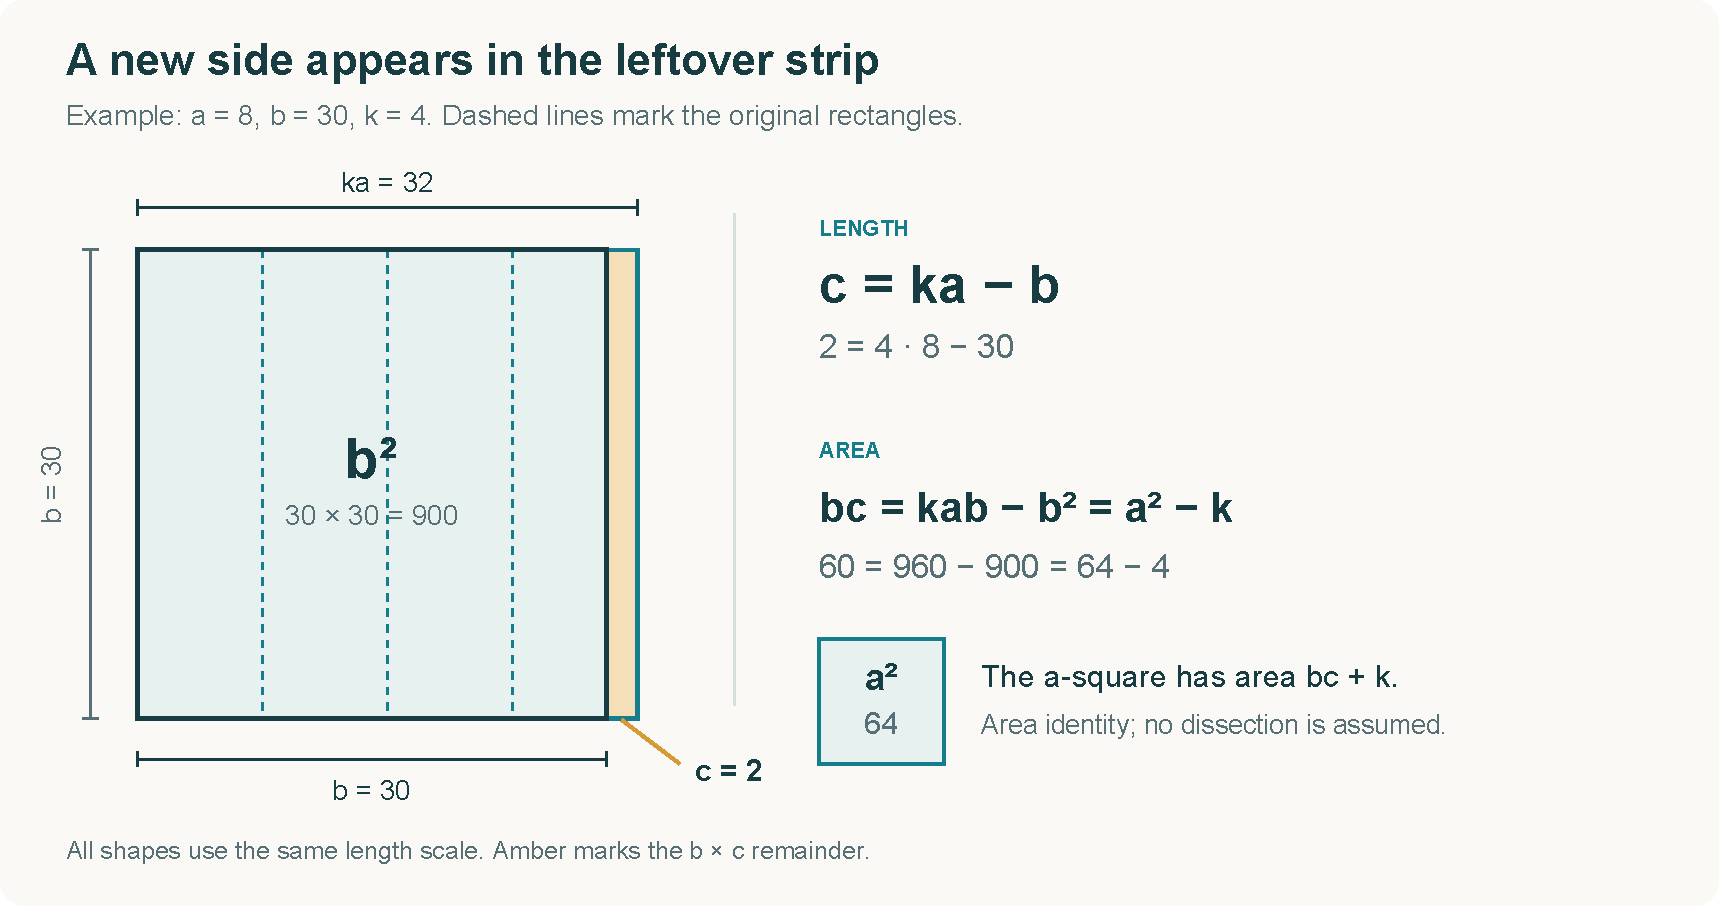
\includegraphics[width=\linewidth]{figures/construction.pdf}
\caption{The strip construction for $(a,b,k)=(8,30,4)$. Four rectangles
form a strip of width $32$; removing the $30$-square leaves width $2$.
The shapes have a common length scale. Equation~\eqref{eq:area} compares
areas; no dissection of the smaller square is asserted.}
\label{fig:construction}
\end{figure}

\section{A worked example}
For $(a,b)=(30,112)$, the quotient is $13444/3361=4$. The complete descent is
\[
 (30,112)\longmapsto(8,30)\longmapsto(2,8)\longmapsto(0,2).
\]
This numerical orbit also appears in Wu's hyperbola visualization~\cite{wu}.
Table~\ref{tab:descent} records the corresponding area identities. The number
of rectangles remains four while the integer lengths decrease.

\begin{table}[htbp]
\centering
\caption{The descent for $k=4$.}
\label{tab:descent}
\medskip
\renewcommand{\arraystretch}{1.2}
\begin{tabular}{@{}cccc@{}}
\hline
Current pair & $c=4a-b$ & $a^2=bc+4$ & Next pair\\
\hline
$(30,112)$ & $8$ & $900=896+4$ & $(8,30)$\\
$(8,30)$ & $2$ & $64=60+4$ & $(2,8)$\\
$(2,8)$ & $0$ & $4=0+4$ & $(0,2)$\\
\hline
\end{tabular}
\end{table}

At the final construction, $ka=b$, so the strip coincides with the
$b$-square. No positive-width rectangle remains, and~\eqref{eq:area}
reduces to $a^2=k$. Figure~\ref{fig:terminal} illustrates this endpoint.
The diagrams use proportional dimensions within each construction;
different constructions may use different scales.

\begin{figure}[htbp]
\centering
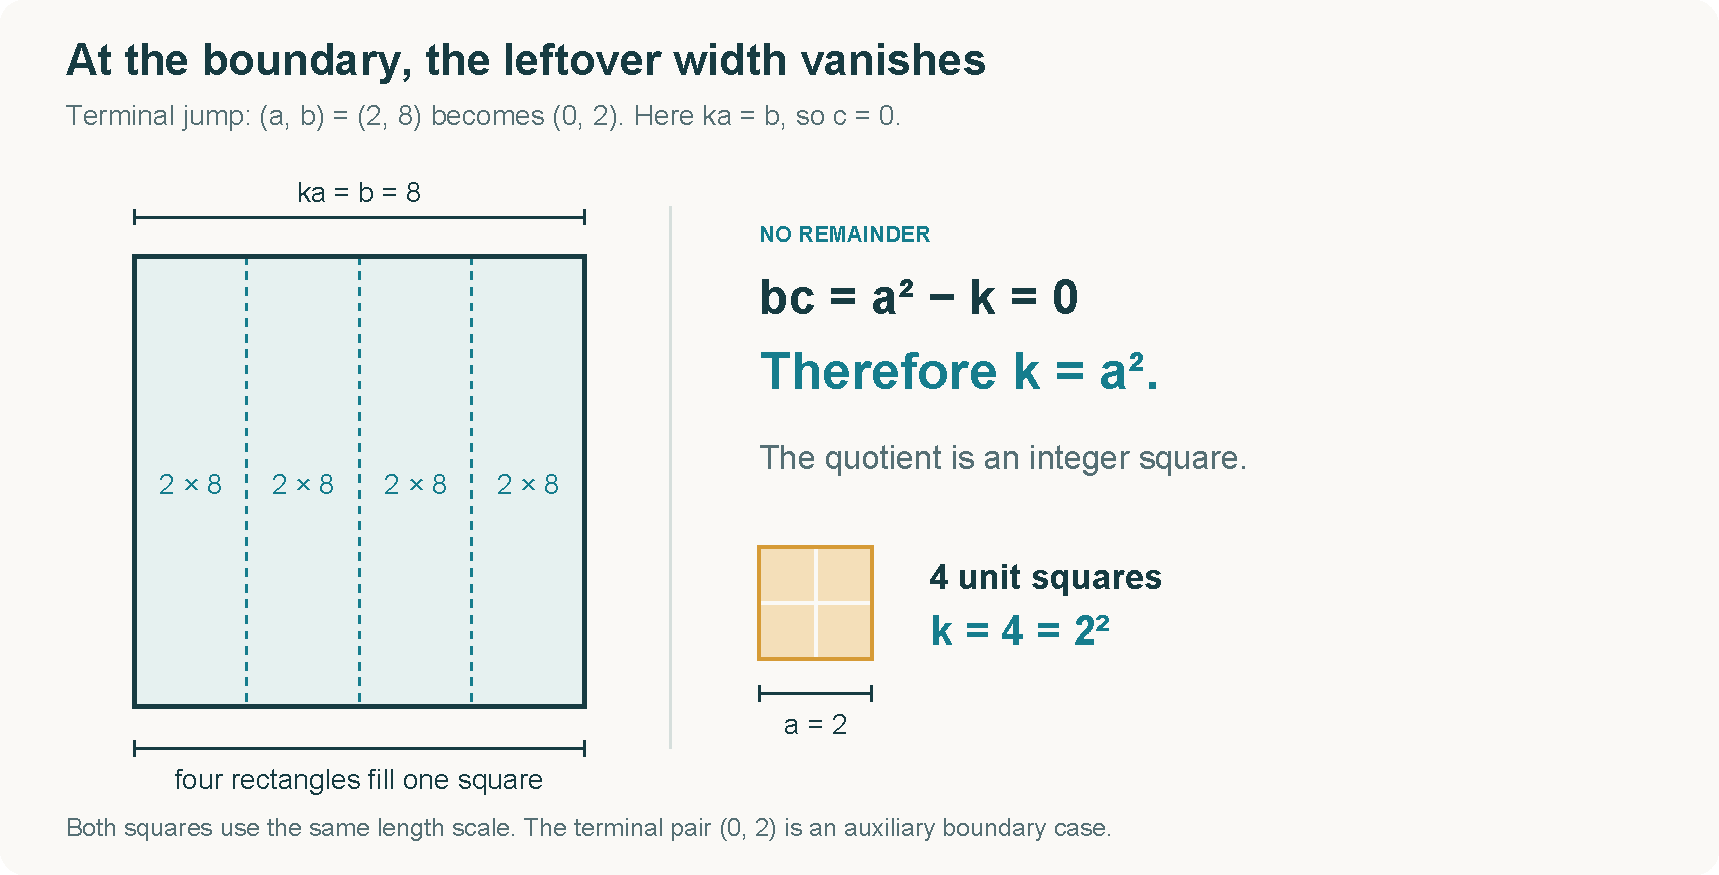
\includegraphics[width=\linewidth]{figures/terminal-case.pdf}
\caption{The final jump $(2,8)\mapsto(0,2)$. Four $2\times8$ rectangles
fill an $8$-square. The accompanying $2$-square, drawn at the same scale,
has area $k=4$.}
\label{fig:terminal}
\end{figure}

\section{Relation to earlier work}\label{sec:context}
Regarding~\eqref{eq:invariant} as a quadratic in its second coordinate gives
\[
 t^2-kat+(a^2-k)=0.
\]
Its roots are $b$ and $ka-b$. Exchanging these roots is the classical
Vieta jump. The strip construction interprets the second root as a
remaining width, while the arithmetic transformation is unchanged.

Campbell's early treatment includes the greatest-common-divisor
conclusion~\cite{campbell}. Wu visualizes Vieta jumping through integer
points on a hyperbola~\cite{wu}. A 2016 online discussion by Moody and
contributors gives a remainder formulation of the same descent and
includes a separate geometric attempt~\cite{moody}; that discussion is
background, not a premise of the proof here.

The contribution of this note is the repeated-rectangle exposition of
that established descent. The references provide context rather than an
exhaustive priority investigation. They do not establish that this
particular area presentation is historically new, and no claim of
priority is made. The argument uses both geometry and integer arithmetic;
the diagrams alone do not prove the theorem.

\section*{Supplementary material}
LaTeX source, SVG diagrams and matching vector PDF exports, diagram-generation
scripts, and finite arithmetic checks are available in the accompanying
repository.\footnote{\url{https://github.com/pranman/imo-1988-6-geometric-proof}}
The README provides a visual exposition
with additional diagrams. The arithmetic script verifies the displayed
examples and all admissible pairs with $1\le a\le b\le400$. These finite
checks can detect transcription errors; the general result follows from
the proof above.

\begin{thebibliography}{9}
\bibitem{imo}
International Mathematical Olympiad.
\emph{1988 problems}, English, Problem 6, 1988.
\href{https://www.imo-official.org/assets/documents/problems/1988/1988_eng.pdf}{Official problem paper}.

\bibitem{campbell}
John Campbell.
A solution to 1988 IMO question 6.
\emph{Mathematics Competitions} \textbf{1}(2) (1988), 29--32.
\href{https://www.wfnmc.org/mc19882campbell.pdf}{Original article}.

\bibitem{wu}
Kyle Wu.
Vieta jumping: visualization and intuition.
\emph{Parabola} \textbf{60}(1) (2024), 1--7.
\href{https://www.parabola.unsw.edu.au/sites/default/files/2024-05/vol60_no1_8.pdf}{Publisher's PDF}.

\bibitem{moody}
Rutger Moody and contributors.
Math Olympiad 1988 problem 6, canonical solution 2 without Vieta jumping.
\emph{Mathematics Stack Exchange}, 29 August 2016.
\href{https://math.stackexchange.com/questions/1906908/math-olympiad-1988-problem-6-canonical-solution-2-without-vieta-jumping}{Question and discussion}.
\end{thebibliography}

\end{document}